\documentclass{article}%
\usepackage[T1]{fontenc}%
\usepackage[utf8]{inputenc}%
\usepackage{lmodern}%
\usepackage{textcomp}%
\usepackage{lastpage}%
\usepackage{authblk}%
\usepackage{graphicx}%
%
\title{Functional EF{-}Hands in Neuronal Calcium Sensor GCAP2 Determine Its Phosphorylation State and Subcellular Distribution In Vivo and Are Essential for Photoreceptor Cell Integrity}%
\author{Stacey Jordan}%
\affil{Department of Veterinary Medicine, School of Veterinary Medicine, National Taiwan University, Taipei, Taiwan, R.O.C., Department of Surgery, Mackay Memorial Hospital, Taipei, Taiwan, R.O.C., Research Institute for Children, Children's Hospital, New Orleans, LA, USA}%
\date{01{-}01{-}2013}%
%
\begin{document}%
\normalsize%
\maketitle%
\section{Abstract}%
\label{sec:Abstract}%
At times, the amygdala, a part of the brain involved in assessing mood, responds to symptoms by activating the hypothalamus, making it more like a suicide bomber firing a faulty gun.\newline%
But in a new study, scientists at the University of Texas at San Antonio discovered that certain blocking proteins inside the hypothalamus can block this response when circulating in the brain. It's a discovery that could give new insight into depression.\newline%
Researchers said they initially suspected that serotonin, the chemical in the brain that increases the activity of the amygdala, might play a role in depression.\newline%
However, when they performed tests on mice, one researcher said the laboratory took on a new perspective.\newline%
"They actually saw that glutamate and this block caused a physical disability," said lead researcher Cathy Muldowney, a professor of psychiatry at the UTSA. "They couldn't recall the day of the week. And when they found out that it was more like what we were seeing, even autism, that much more of an explanation."\newline%
Muldowney worked with UCSD Professor Chris Angeloff to find the potential blockers of the glutamate, and two proteins in their system, called "Neuronal Panx1" and "Neuronal Pulse" were finally explained.\newline%
"It's almost impossible to activate these proteins without injuring neurons in the hypothalamus, and our view is that, in the long run, that might be important to these symptoms of depression," Muldowney said.\newline%
The study will be published in the March edition of Science.

%
\subsection{Image Analysis}%
\label{subsec:ImageAnalysis}%


\begin{figure}[h!]%
\centering%
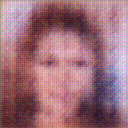
\includegraphics[width=150px]{500_fake_images/samples_5_260.png}%
\caption{A Man With A Beard Wearing A Tie}%
\end{figure}

%
\end{document}